\documentclass{sigchi-ext}
% Please be sure that you have the dependencies (i.e., additional
% LaTeX packages) to compile this example.
\usepackage[T1]{fontenc}
\usepackage{textcomp}
\usepackage[scaled=.92]{helvet} % for proper fonts
\usepackage{graphicx} % for EPS use the graphics package instead
\usepackage{balance}  % for useful for balancing the last columns
\usepackage{booktabs} % for pretty table rules
\usepackage{ccicons}  % for Creative Commons citation icons
\usepackage{ragged2e} % for tighter hyphenation
\usepackage[utf8]{inputenc} % for a UTF8 editor only

\copyrightinfo{Permission to make digital or hard copies of all or
part of this work for personal or classroom use is granted without
fee provided that copies are not made or distributed for profit or
commercial advantage and that copies bear this notice and the full
citation on the first page. Copyrights for components of this work
owned by others than ACM must be honored. Abstracting with credit is
permitted. To copy otherwise, or republish, to post on servers or to
redistribute to lists, requires prior specific permission and/or a
fee. Request permissions from permissions@acm.org.\\
{\emph{CHI'14}}, April 26--May 1, 2014, Toronto, Canada. \\
Copyright \copyright~2014 ACM ISBN/14/04...\$15.00. \\
DOI string from ACM form confirmation}

% Paper metadata (use plain text, for PDF inclusion and later
% re-using, if desired).  Use \emtpyauthor when submitting for review
% so you remain anonymous.
\def\plaintitle{Emotion-based music recommendation using supervised learning}
\def\plainauthor{Karl-Arnold Bodarwé, Philipp Jean-Jacques, Jenny Noack}
\def\emptyauthor{}
\def\plainkeywords{music recommendation;music emotion;supervised learning;naive bayes;mfcc;rms;chroma;}
\def\plaingeneralterms{Music Recommendation}

\title{Emotion-based music recommendation using supervised learning}

\numberofauthors{3}
% Notice how author names are alternately typesetted to appear ordered
% in 2-column format; i.e., the first 4 autors on the first column and
% the other 4 auhors on the second column. Actually, it's up to you to
% strictly adhere to this author notation.
\author{%
  \alignauthor{%
    \textbf{Karl-Arnold Bodarwé}\\
    \affaddr{University of Regensburg} \\
    \affaddr{Regensburg, Bayern, 93053, Germany} \\
    \affaddr{karl-arnold.bodarwe@stud.uni-regensburg.de} }\alignauthor{%
    \textbf{Jenny Noack}\\
    \affaddr{University of Regensburg} \\
    \affaddr{Regensburg, Bayern, 93053, Germany} \\
    \affaddr{jenny.noack@stud.uni-regensburg.de} } \vfil \alignauthor{%
    \textbf{Philipp Jean-Jacques}\\
    \affaddr{University of Regensburg} \\
    \affaddr{Regensburg, Bayern, 93053, Germany} \\
    \affaddr{philipp.jean-jacques@stud.uni-regensburg.de} }\alignauthor{%
  }
}
% Make sure hyperref comes last of your loaded packages, to give it a
% fighting chance of not being over-written, since its job is to
% redefine many LaTeX commands.
\definecolor{linkColor}{RGB}{6,125,233}
\hypersetup{%
  pdftitle={\plaintitle},
  pdfauthor={\plainauthor},
  pdfkeywords={\plainkeywords},
  bookmarksnumbered,
  pdfstartview={FitH},
  colorlinks,
  citecolor=black,
  filecolor=black,
  linkcolor=black,
  urlcolor=linkColor,
  breaklinks=true,
}

\begin{document}

\maketitle

% Uncomment to disable hyphenation (not recommended)
% https://twitter.com/anjirokhan/status/546046683331973120
\RaggedRight{}

\begin{abstract}
Music recommendation systems are well explored and commonly used but are normally based on
manually tagged parameters and simple similarity calculation. Our project proposes a recommendation system based on emotional computing, automatic classification and feature extraction, which recommends music based on the emotion expressed by the song.\\
To achieve this goal a set of features is extracted from the song, including the MFCC (mel-frequency cepstral coefficients) following the works of McKinney et al. \cite{Mckinney2003} and a machine learning system is trained on a set of 424 Songs, which are categorized by emotion. The categorization of the song is performed manually by multiple persons to avoid error. The emotional categorization is performed using a modified version of the Tellegen-Watson-Clark emotion model \cite{Tellegen1999}, as proposed by Trohidis et al. \cite{Trohidis2011}.
The System is intended as desktop application that can reliably determine similarities between the main emotion in multiple pieces of music, allowing the user to choose music by emotion. We report our findings below.
\end{abstract}

\keywords{\plainkeywords}

\category{H.3.2}{Record classification}{Miscellaneous}

\section{Introduction}
Musical Recommender systems are well known and widespread. Using methods such as tags or similar user behaviour, pieces of music can be recommended by a variety of features.\\
Music and emotion are strongly related to each other \cite{Krumhansl2002} but emotion is never considered in existing recommender systems. To try a new approach to recommending music, we decided to implement a system that recommends music by emotion. The emotion of the song is determined using a classifier that is trained on audio-features extracted from the song. The extracted emotion is then used to recommend a song to the user.

\begin{marginfigure}[0pc]
  \begin{minipage}{\marginparwidth}
    \centering
    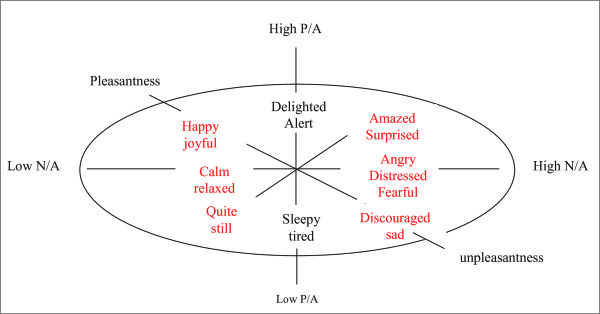
\includegraphics[width=1.0\marginparwidth]{images/tellegen-watson-clark-model.png}
    \caption{Tellegen-Watson-Clark model of mood \cite{Tellegen1999}}~\label{fig:tellegen-watson-clark}
  \end{minipage}
\end{marginfigure}

\section{Related Work}
There have been various approaches on how to classify a piece of music by its emotion. There are different emotion models used as well as different feature extraction techniques.

\subsection{Emotion Models}
In multiple models emotion is mapped as a matrix where the axes relate to a certain emotional aspect and adjectives are placed in a circle inside the matrix to provide a guide. The number of axes varies from model to model and even in certain implementations of a model itself.\\
The Tellegen-Watson-Clark model, as used by \cite{Trohidis2011} has two axes labeled Positive Affect and Negative Affect which are used to show correlations between them and map emotions accordingly. Another dimension that can be derived from this model is the level of pleasantness of a certain emotion.\\

Other projects use the Valence Arousal model, a similar approach. The axes are labeled \textit{Valence} and \textit{Arousal}, with \textit{Valence} describing the happiness of the emotion and \textit{Arousal} describing the state of agitation entered by the emotion. The mapping of the adjectives to the matrix look similar to the Tellegen-Watson-Clark model, although the axes have different meanings.

\subsection{Feature Extraction and Classification}
Different researchers have tried different approaches to classification of music, not necessarily for classification of emotion. \cite{Mckinney2003} have proposed a method to automatically determine the genre of a certain piece of audio, including noise and speech. They tested different methods of classification against each other, resulting in good values for MFCC Analysis as well as Psychoacoustic features and a set of features called auditory filter temporal envelope, a set of bandpass filters which mimics the range of hearing of a human ear.\\

\cite{Li2003} give a comparison of classification techniques for automatic assignment of genres, including MFCC, FFT, Beat and Pitch, showing best results for FFT and MFCC, or a combination of these with other features. They make use of a Support Vector Machine for classifying, with good results.
\cite{Tzanetakis2001} also focus on the automatic classification of genres, focusing on the calculation of certain features such as STFT (short time fourier transform) and MFCC. The paper shows how to calculate the different features and explains the results. They find the best results when working with MFCC and STFT and identify genres that are harder to distinguish than others.

\section{Emotion Model}
To be able to distinguish between emotions more easily, we decided to use a simplified version of the Tellegen-Watson-Clark model. We defined four emotional categories, marking the extreme ends of the graphs used in the model. The categories proposed in the Tellegen-Watson-Clark model have some adjectives that are very similar and difficult to distinguish especially when dealing with music as a carrier of emotion. Categories such as \textit{calm-relaxing} and \textit{quiet-still}, or \textit{amazed-surprised} and \textit{happy-pleased} were combined into one category. The remaining categories are:

\begin{itemize}
	\item calm-relaxing
	\item happy-amazed
	\item angry-fearful
	\item sad-lonely
\end{itemize}

\begin{marginfigure}[0pc]
  \begin{minipage}{\marginparwidth}
    \centering
    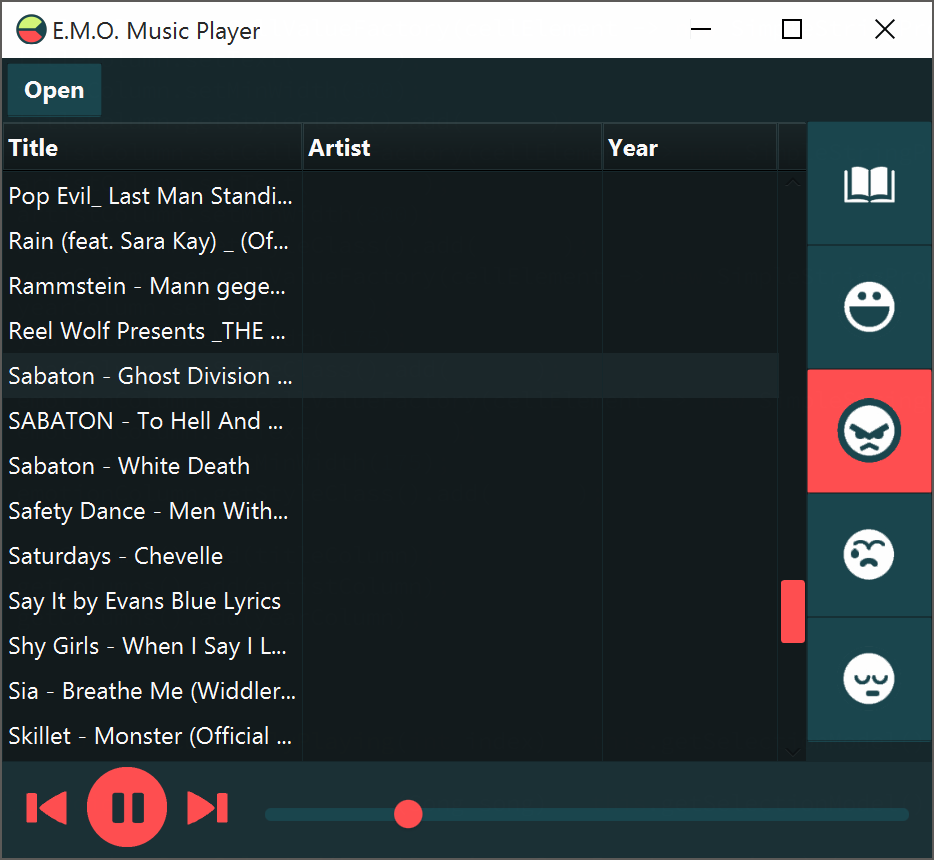
\includegraphics[width=1.0\marginparwidth]{images/screenshot.png}
  	\caption{User interface of the music player}~\label{fig:screenshot}
  \end{minipage}
\end{marginfigure}

\section{Training Data}\label{training-data}
To create a the training data for the classifier, we accumulated a collection of 424 songs of various genre and artist, roughly sorted by their main emotion, by searching various online streaming and video platforms, such as Youtube and Spotify for playlists with tags fitting our emotional model.\\
Those songs were then tagged by 3 independent raters into the four emotional categories mentioned above. Afterwards \textit{Fleiss' Kappa} was calculated over the results, to use only songs for the creation of the training data where all raters agreed on the same emotion. The following table schows the distribution of kappa values over all songs.\\

\begin{table}
  \centering
  \label{kappa-distribution}
  \begin{tabular}{@{}lll@{}}
    Kappa & Count & Percent \\ \midrule
    1.00 & 260 & 61.32\% \\
    0.33 & 155 & 36.56\% \\
    0.00 & 9 	 & 2.12\%
  \end{tabular}
  \caption{Distribution of Kappa values across tagged values}
\end{table}

Most of the disagreement (90 songs) were in categories \textit{calm-relaxing} and \textit{sad-lonely}, predicting difficulties in the differentiation of these categories.\\

To try to get an overview about useful features we processed a small sample of audio files with the jAudio feature extractor \cite{McEnnis2005}, extracting as many features as possible.
Previous research on which features to use for audio classification has shown that MFCC, along with several low level features, such as RMS, where showing promising results and we decided to use these features for our classification.\cite{Mckinney2003, Mandel2005, Tzanetakis2001}.  Because the application is meant to be used in real time, the feature extraction needs to be as quickly as possible. Therefore as few features as possible were used without impairing the classification too much. The final feature vector consists of 26 features.

\begin{table}
  \centering
  \begin{tabular}{@{}ll@{}}
    Feature Count & Feature Name \\ \midrule
    13 & MFCC \\
    12 & Chroma \\
    1  & RMS
  \end{tabular}
  \caption{Feature vector}
  \label{feature-vector}
\end{table}

\section{System}
The audio processing library we used was \textit{jAudio} \cite{McEnnis2005}, a gui application specifically developed for feature extraction. This application is written in Java and supports both wav and mp3 formats.\\
The system was implemented as a simple Music Player. The user interface provides a set of buttons associated with the emotions, which allow the user to filter the available songs by their emotion. A song is classified as soon as it is loaded into the music library of the player.\\
The classification is done by a Naive Bayes classifier, because it showed the best performance in comparison to the other classifiers tested (Support Vector Machine, Logistic Regression, Decision Trees).

\section{Results}
The classifier was trained using the training data explained in the "Training Data" section and evaluated using 10-fold cross validation. The classifier seems to perform poorly given that only 54.07\% of all songs could be correctly classified, but having in mind that human raters assigned to only 61.32\% of all songs the same label, the classifier performs very well. The results also show, that the emotion of a song is a highly subjective experience and may need additional input data, like analysis of lyrics or additional audio features to become more precisely determinable.

\begin{table}
  \centering
  \begin{tabular}{@{}lll@{}}
    Correctly Classified          & 138       & 53.07\% \\
    Incorrectly Classified        & 122       & 46.93\% \\
    Kappa statistic               & 0.35      & \\
    Mean absolute error           & 0.23      & \\
    Root mean squared error       & 0.45      & \\
    Relative absolute error       & 64.52\%   & \\
    Root relative squared error   & 105.10\%  & \\
    Total Number of Instances     & 260       & 100\%
  \end{tabular}
  \caption{Evaluation of the Naive Bayes classifier}
\end{table}

In the process of the project, we have come to a few conclusions regarding methods and tools. We used the jAudio library to get an overview of available features, but struggled with the documentation of the code during the implementation. While jAudio has an easy to use graphical user interface for feature extraction, which can create great amounts of usable data in little time, the possibility to embed the application into a system is lacking.

\section{Conclusion}
We found that it is possible to classify music via emotion and build a recommending system around that classification. With further refinement of the extracted features and possibly the addition of non-musical features such as lyrics, we are positive that the accuracy of the classification can be further improved. A recommendation system such as this could, for example, be trained on the large library of a streaming platform and built into the player, as a new and unique way to find music.

\bibliographystyle{SIGCHI-Reference-Format}
\bibliography{literature}

\end{document}
